% -----------------------------------------------------------------------------
% Implementation
% -----------------------------------------------------------------------------
\chapter{Implementation}
\label{chap:implementation}
\section{Image Source Method}
The implementation of the image source model will unfold in several steps. Building up from a rudimentary to a more complex and realistic implementation.
\subsection{Images Source Model with 4 walls - image order 1}
We start by modeling a simple room with only 4 walls (no ceiling or floor) with a receiver positioned at the point (single source positioned at the point $P(1,1,1)$ and its reflection of the first order relative to the walls as seen in figure \ref{fig:ism_4_1_geo}\\
\begin{figure}
    \centerline{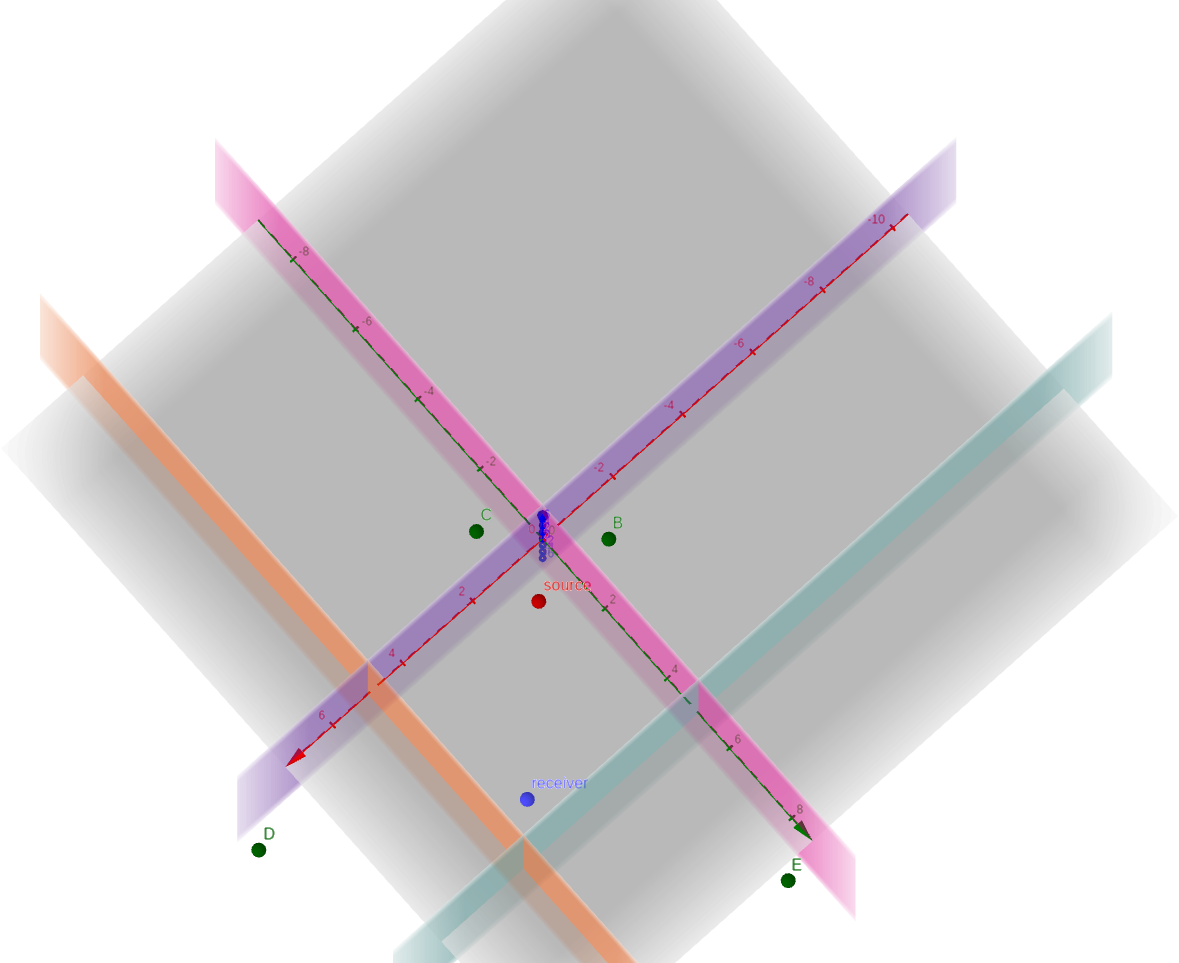
\includegraphics[width=1.3\textwidth,keepaspectratio]{LaTeX/images/geometrie/ism_4_walls_order_1.png}}
    \caption{Source and receiver in room with 4 walls and reflections of order 1}
    \label{fig:ism_4_1_geo}
\end{figure}
When adding the pressure waves emitted by the source and all the source images we get the pressure deviation perceived at the receiver as seen in figure \ref{fig:ism_4_1_mat}
\begin{figure}

    \centerline{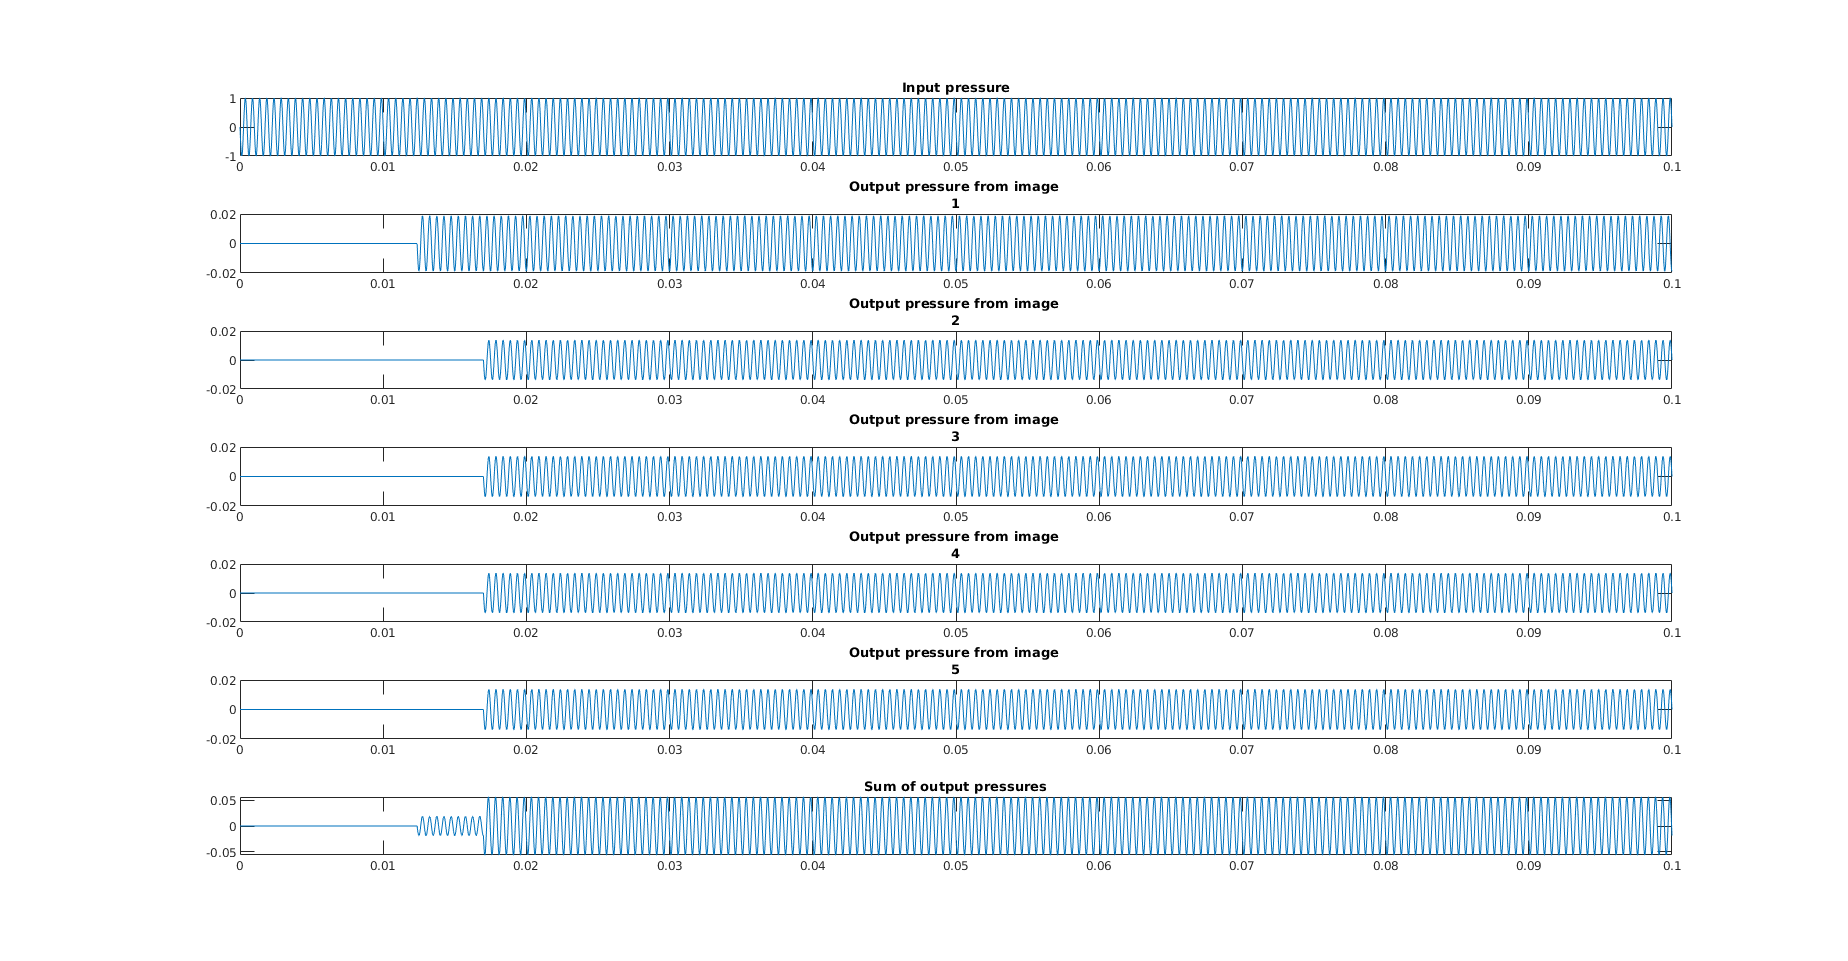
\includegraphics[width=1.8\textwidth,keepaspectratio]{LaTeX/images/plots/matlab_4_walls_order_1.png}}
    \caption{Pressure deviation perceived at receiver emitted by source and source images}
    \label{fig:ism_4_1_mat}
\end{figure}
\newpage
In the next step the same scenario is computed for an image order 2. Each image is produces itself one image relative to each wall as seen in figure \ref{fig:ism_4_2_geo}\\
\begin{figure}
    \centerline{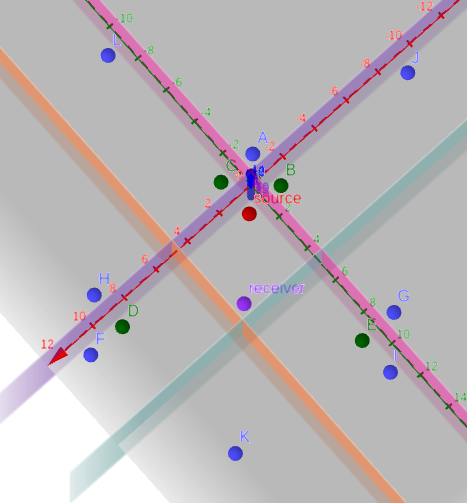
\includegraphics[width=1.3\textwidth,keepaspectratio]{LaTeX/images/geometrie/ism_4_walls_order_2.png}}
    \caption{Source and receiver in room with 4 walls and reflections of order 1}
    \label{fig:ism_4_2_geo}
\end{figure}